%-------------------------------------------------------------------------------
% seq64_song_editor
%-------------------------------------------------------------------------------
%
% \file        seq64_song_editor.tex
% \library     Documents
% \author      Chris Ahlstrom
% \date        2015-08-31
% \update      2017-09-30
% \version     $Revision$
% \license     $XPC_GPL_LICENSE$
%
%     Provides the concepts.
%
%-------------------------------------------------------------------------------

\section{Song Editor}
\label{sec:seq64_song_editor}

   The \textsl{Sequencer64 Song Editor} is used to combine all of the patterns
   into a complete tune.  It works by showing one row per
   pattern/loop/sequence in numbered columns, and the placement of each
   pattern at various musical bars in the song.
   \index{performance}
   In \textsl{Sequencer64} parlance, the Song Editor creates a
   \textsl{performance}.
   \index{song mode}

   \textbf{New:}
   \index{new!dual song editors}
   As an option in the \texttt{[user-interface]}
   section of the "user" configuration file, two song editor windows can be
   brought onscreen, as a convenience for arranging projects with a large
   number of sequences/patterns.
   It also provides the "song mode" of \textsl{Sequencert64},
   as opposed to the "live mode" provided by the Patterns Panel, when
   \textsl{Sequencer64} is running in ALSA mode.
   (In JACK mode, the live versus song mode is controlled by the JACK start-mode
   flag.)

   When the Song Editor has the focus of the application, in ALSA mode, it
   takes over control from the Patterns Panel.  The Song Editor then
   controls playback.  Once playback is started in the Song Editor, some actions
   in the Patterns Panel no longer have effect, effectively disabling live
   mode.  The Song Editor takes over the arming/unarming (unmuting/muting)
   shown in the Patterns Panel.  The highlighting of armed/unarmed patterns
   changes according to whether the pattern is playing in the Song Editor, or
   not.  If one tries to change the muting using a hot-key (or even a click) in
   the Patterns Panel, the Song Editor immediately returns the pattern to the
   state it has in the Song Editor.  The only way to manually change the muting
   then is to click the pattern's label in the Song Editor.
   
   Both the Song Editor and the Patterns Panel both reflect the change in
   muting in the user interface, though with \textsl{opposite colors}.

\begin{figure}[H]
   \centering 
%  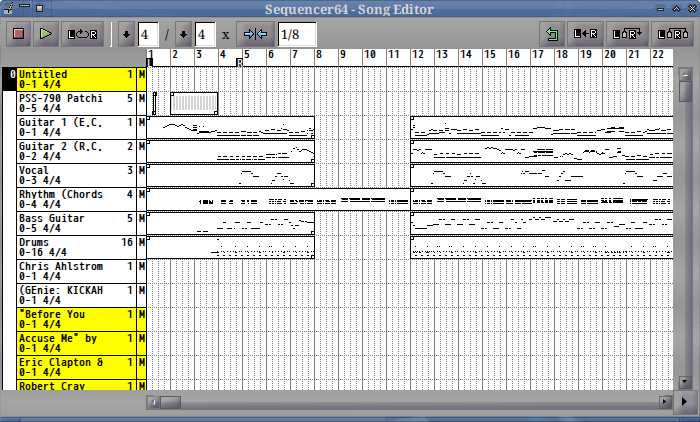
\includegraphics[scale=0.75]{song-editor/song-editor-window-new.png}
%  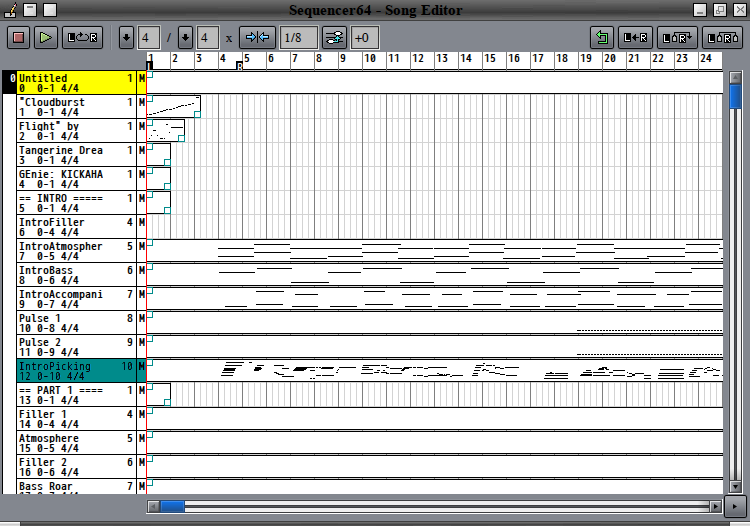
\includegraphics[scale=0.75]{new/song_editor_transpose-0_9_15.png}
   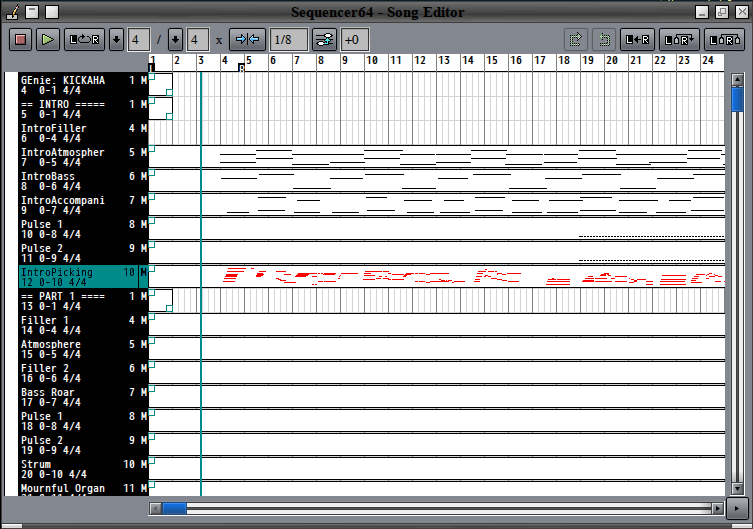
\includegraphics[scale=0.75]{song-editor/song-editor-window.png}
   \caption{Song Editor Window}
   \label{fig:song_editor_window}
\end{figure}

   \textbf{New:}
   There are some new features for the song editor, as
   seen above and in the following figure:

\begin{figure}[H]
   \centering 
   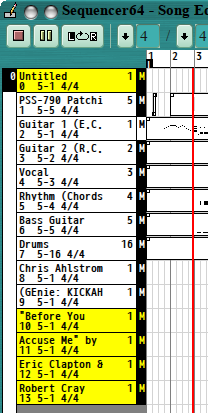
\includegraphics[scale=0.75]{new/song-editor-0_9_10_1.png}
   \caption{Song Editor Window, New Features}
   \label{fig:song_editor_window_new_features}
\end{figure}

   \begin{itemize}
      \index{shift left click}
      \item Toggling of the mute state of multiple patterns by holding the
         Shift key while left-clicking on the M or a pattern name;
      \index{pause}
      \item The new Pause button functionality;
      \index{progress bar}
      \item The optional coloring (about 7 color values are selectable)
         and thickening of the progress bar.
      \index{redo}
      \item A new Redo button (not shown).
      \index{transpose}
      \item A new Transpose button (not shown).
      \index{untransposable color}
      \item Red coloring of events for patterns that are not transposable, such
         as drum tracks.
   \end{itemize}

   \index{new!empty pattern}
   \textbf{New:} 
   This dialog (in \textsl{Sequencer64}) shows any empty patterns
   highlighted in yellow.  An empty pattern is one that exists, but
   contains only meta information, and contains no MIDI events that
   can be played.  For example, some tracks just serve as name tracks or
   information tracks.
   
   The Song Editor is not too complex, but for exposition, we break it into
   the top panel, the bottom panel, and the rest of the window.

   \textbf{New:}
   There are still more features of the song editor in
   pending version 0.9.15, as seen in the following
   figure:

\begin{figure}[H]
   \centering 
   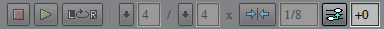
\includegraphics[scale=0.75]{new/song_editor_top_panel_transpose-0_9_15.png}
   \caption{Song Editor Window, Transpose Song}
   \label{fig:song_editor_window_transpose_song}
\end{figure}

   \index{transpose}
   Notice the additional button that allows the whole song (except for
   exempt, non-transposable sequences) to be transposed up or down by up to an
   octave in either direction.

\subsection{Song Editor / Top Panel}
\label{subsec:seq64_song_editor_top}

   The top panel provides quick access to song-playback actions and
   configuration.

\begin{figure}[H]
   \centering 
%  \includegraphics[scale=0.55]{song-editor/song-editor-top-panel-items.png}
   \includegraphics[scale=0.55]{new/song-editor-top-panel-items.png}
   \caption{Song Editor / Top Panel Items}
   \label{fig:song_editor_top_panel_items}
\end{figure}

   \begin{enumber}
      \item \textbf{Stop}
      \item \textbf{Play}
      \item \textbf{Play Loop}
      \item \textbf{Beats Per Bar}
      \item \textbf{Beat Unit}
      \item \textbf{Grid Snap}
      \item \textbf{Transpose}
      \item \textbf{Toggle JACK Sync}
      \item \textbf{Toggle Following JACK Transport}
      \item \textbf{Redo}
      \item \textbf{Undo}
      \item \textbf{Collapse}
      \item \textbf{Expand}
      \item \textbf{Expand and copy}
   \end{enumber}

   \setcounter{ItemCounter}{0}      % Reset the ItemCounter for this list.

   \itempar{Stop}{song editor!stop}
   Stops the playback of the song.
   \index{keys!esc (stop)}
   The keystroke for stopping playback is the \texttt{Escape} character.
   It can be configured to be another character (such as \texttt{Space}, which
   would make the space-bar toggle the playback status).

   \itempar{Play}{song editor!play}
   \index{L marker}
   Starts the playback of the song, starting at the \textbf{L marker}.
   The \textbf{L marker} serves as the start position for playback
   in the Song Editor.  One can change the start position only when the
   performance is not playing.
   \index{keys!space (play)}
   The default keystroke for starting playback is the \texttt{Space} character.
   \index{keys!esc (stop)}
   The default keystroke for stopping playback is the \texttt{Escape} character.
   \index{keys!period (pause)}
   The default keystroke for pausing playback is the \texttt{Period} character,
   which currently works only in ALSA mode.

   \itempar{Play Loop}{song editor!play loop}
   \index{loop mode}
   Activate loop mode. When Play is activated,  play the song and loop
   between the
   \index{L marker}
   \index{R marker}
   \textbf{L marker} and the \textbf{R marker}.
   This button is a state button, and its appearance indicates when it is
   depressed, and thus active.
   If this button is deactivated during playback, then playback will
   continue past the \textbf{R marker}.

   \itempar{Beats Per Bar}{song editor!beats/bar}
   Part of the time signature, and specifies the number of beat units per bar.
   The possible values range from 1 to 16.

   \itempar{Beat Unit}{song editor!beat unit}
   Also called "beat width".
   Part of the time signature, and specifies the size of the beat unit:
   1 for whole notes; 2 for half notes; 4 for quarter notes; 8 for eight notes;
   and 16 for sixteenth notes.

   \itempar{Grid Snap}{song editor!grid snap}
   Grid snap selects where the patterns will be drawn.
   Unlike the \textbf{Grid Snap} of the Pattern Editor, the units
   of the Song Editor snap value are in fractions of a measure length.
   The following values are supported:
   1, 1/2, 1/4, 1/8, 1/16, 1/32, and 1/3, 1/6, 1/12, and 1/24.

   \itempar{Redo}{song editor!redo}
   The Redo button will reapply the last change that was "undone" by
   the Undo button.
   It will be inactive if there is nothing to redo.

   \itempar{Undo}{song editor!undo}
   The Undo button will roll back the last change in the layout of a
   pattern.  Each time it is clicked, the most recent change will be undone.
   It will roll back one change each time it is pressed.
   It is not certain what the undo limit is, however.
   It will be inactive if there is nothing to undo.

   \itempar{Collapse}{song editor!collapse}
   This button collapses the song between the \textbf{L marker} and the
   \textbf{R marker}.
   What this means is that, if there is song material (patterns) before the
   \textbf{L marker} and after the \textbf{R marker},
   and the \textbf{Collapse} button is
   pressed, any song material between the L and R markers is wiped out, and
   the song material after the \textbf{R marker} is moved leftward to
   the \textbf{L marker}.
   Collapsing occurs in all tracks present in the Song Editor.

   \itempar{Expand}{song editor!expand}
   This button expands the song between the
   \textbf{L marker} and the \textbf{R marker}.
   It inserts blank space between these markers, moving the song material
   that is after the \textbf{R marker}
   to the right by the duration of the blank space.
   Expansion occurs in all tracks present in the Song Editor.

   \itempar{Expand and copy}{song editor!expand and copy}
   This button expands the song between the \textbf{L marker} and the
   \textbf{R marker} much like the \textbf{Expand} button.
   However, it also copies the original data that is present after the
   \textbf{R marker}, and pastes it into the newly-available space between
   the L and R markers.

\subsection{Song Editor / Arrangement Panel}
\label{subsec:seq64_song_editor_arrangement_panel}

   The arrangement panel is the middle section shown in
   \figureref{fig:song_editor_window}.  It is also known as the
   "piano roll" of the song editor. Here, we zero in on its many
   features.

   Keystrokes and additional mouse configuration have been added to make
   editing easier even without a good mouse.
   For example, one can page up and down vertically in the arrangement
   panel using the
   \index{keys!page-up} Page Up and 
   \index{keys!page-down} Page Down keys.
   One can go to the top using the 
   \index{keys!home} Home key,
   to the bottom using the
   \index{keys!end} End key.
   One can page left and right horizontally in the arrangement
   panel using the
   \index{keys!shift-page-up} Shift Page Up and 
   \index{keys!shift-page-down} Shift Page Down keys.
   One can go to the leftmost position using the 
   \index{keys!shift-home} Home key,
   and to the rightmost position using the
   \index{keys!shift-end} End key,

   The following figure is taken from a conventional MIDI file, imported,
   with a few long tracks, rather than a large number of smaller patterns.
   In other words, the patterns used here are very long, and used only once
   in the song.
   (We will provide an example that shows off \textsl{Sequencer64}'s
   pattern features better, at some point.)

   Please note that, if playback is started with the Song Editor as the
   active window, then the pattern boxes in the patterns panel will
   show as armed/unarmed (unmuted/muted) depending upon whether or not the
   pattern is shown as playing (or not) at the current playback position in
   the Song Editor piano roll.

   The following figure highlights the main features of the center panel of the
   song editor.

\begin{figure}[H]
   \centering 
   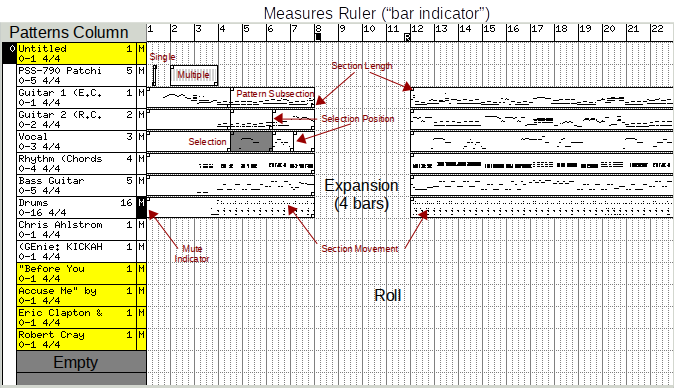
\includegraphics[scale=0.75]{song-editor/song-editor-window-full-items.png}
   \caption{Song Editor Arrangement Panel, Annotated}
   \label{fig:song_editor_window_full_items}
\end{figure}

   \index{transpose}
   One new feature of the song editor is that, if the new Transpose feature is
   built into \textsl{Sequencer64}, any patterns that are marked as exempt from
   transposition (common with drum tracks) have their events shown in red
   instead of black.

\begin{figure}[H]
   \centering 
   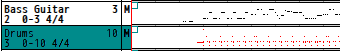
\includegraphics[scale=1.0]{new/perf-non-transposable.png}
   \caption{Song Editor for Non-Transposable Patterns}
   \label{fig:song_editor_non_transposable_items}
\end{figure}

   \index{measures ruler}
   The measures ruler (measures strip)
   consists of a \textsl{measures ruler} (bar indicator) at the top, a
   numbered patterns column at the left with a muting indicator, and the
   grid or roll section.  There are a lot of hidden details in the
   arrangement panel, as the figure shows.  Here are the main sections we
   will deal with:

   \begin{enumber}
      \item \textbf{Patterns Column}
      \item \textbf{Piano Roll}
      \item \textbf{Measures Ruler}
   \end{enumber}

   These items are discussed in the following sections.

\subsubsection{Song Editor / Arrangement Panel / Patterns Column}
\label{subsubsec:seq64_song_editor_arrangement_panel_patterns_column}

   Here are the items to note in the patterns column:

   \begin{enumber}
      \item \textbf{Number}.
         Not yet sure what the number on the left means.
         The number of the screen set?
      \item \textbf{Title}.
         \index{pattern!title}
         \index{pattern!name}
         The title is the name of the pattern, for easy reference.
      \item \textbf{Channel}.
         \index{pattern!channel}
         The channel number appears (redundantly)
         at the right of the title.
      \item \textbf{Buss-Channel}.
         \index{pattern!buss-channel}
         This pair of numbers shows the MIDI buss number used in the pattern
         and the channel used for the pattern.
      \item \textbf{Beat/Measure}.
         \index{pattern!beat}
         This pair of numbers is the standard time-signature of the pattern.
      \item \textbf{Mute Indicator}.
         \index{song editor!mute indicator}
         The letter M is in a black box if the track/pattern is muted, and a
         white box if it is unmuted.
         Left-clicking on the "M" (or the name of the pattern)
         will mute/unmute the pattern.
         \index{shift left click}
         If the Shift key is held while left-clicking on the M or the pattern
         name, then
         the mute/unmute state of every other active pattern is toggled.
         This feature is useful for isolating a single track or pattern.
      \item \textbf{Empty Track}.
         Completely empty tracks (no track events or meta events)
         are indicated by a dark-gray filling in the pattern column.
         Tracks that have only meta information, but no playable event, are
         indicated by a yellow filling in the pattern column.
   \end{enumber}

   The patterns column shows a list of all of the patterns that have been
   created in the current song.  Each pattern in this list has a track of
   pattern layouts associated with it in the piano roll section.

   \index{patterns column!left click}
   \index{song editor!muting}
   Left-clicking on the pattern name or the "M" button toggles the muting
   (arming) status of the track.

   \index{patterns column!ctrl left click}
   \index{song editor!inverse muting}
   Shift-left-clicking on the pattern name or the "M" button toggles the muting
   (arming) status of \textsl{all other tracks} except the track that was
   selected.  This action is useful for quickly listening to a single sequence
   in isoloation.

   \index{patterns column!right click}
   Right-clicking on the pattern name or the "M" button brings up the same
   pattern editing menu as discussed in
   \sectionref{subsubsec:seq64_patterns_pattern_filled}.
   Recall that this context menu has the following entries:
   \textbf{Edit...}, \textbf{Event Edit...}, \textbf{Cut}, \textbf{Copy},
   \textbf{Song}, \textbf{Disable Transpose}, and \textbf{MIDI Bus}.

\subsubsection{Song Editor / Arrangement Panel / Piano Roll}
\label{subsubsec:seq64_song_editor_arrangement_panel_roll}

   The "Piano Roll" section of the arrangement panel is where patterns or
   subsections are inserted, deleted, shrunk, lengthened, or moved.
   Here are the items to note in the annotated Piano Roll area
   shown in \figureref{fig:song_editor_window_full_items}:

   \begin{enumber}
      \item \textbf{Single}.
         In the diagram, under the word "Single", is a very small pattern.
         It is small because it consists only of some MIDI Program Change
         messages meant to set the programs on a Yamaha PSS-790 keyboard.
      \item \textbf{Multiple}.
         This item is the same pattern as in "Single", but dragged out for
         multiple repetitions, simply to show how even the shortest patterns
         can be replicated easily.
      \item \textbf{Pattern Subsection}.
         \index{song editor!middle click}
         \index{pattern subsection}
         Middle-clicking inside a pattern inserts a selection position
         marker in it, breaking the pattern into two equal pieces.
         We call each piece a \textsl{pattern subsection}.
         This division can be done over and over.
         (Note that, in the Song Editor, a middle-click
          \textsl{cannot} be simulated by ctrl-left-click.)
      \item \textbf{Selection Position}.
         A selection position is a marker that divides a pattern into two
         pieces, called \textsl{pattern subsections}.  This makes it easy to
         select smaller portions of a pattern for editing or deleting.  It
         is especially useful for making holes in a pattern.  There may be
         other uses of a selection position that we have not yet discovered.
      \item \textbf{Selection}.
         By clicking inside a pattern or a pattern subsection, it darkens
         (gray) to denote that it is selected.
         A pattern subsection can be deleted by the
         \index{keys!delete}
         Delete key, copied by the
         \index{keys!ctrl-c}
         \index{keys!copy}
         \texttt{Ctrl-C} key, and then inserted (one or more times) by the
         \index{keys!ctrl-v}
         \index{keys!paste}
         \texttt{Ctrl-V} key.  When inserted, each insert goes immediately
         after the current item or the previous insertion.  The same can be
         done for whole patterns.
      \item \textbf{Section Length}.
         \index{song editor!handle}
         \index{song editor!section length}
         Looking closely at the diagram where the arrows point, small
         squares in two corners of the patterns can be seen.  By grabbing
         that square with a left-click, the square can be moved horizontally
         to either lengthen or shorted the pattern or pattern subsection, if
         there is room to move in the desired direction.
         It doesn't matter if the item is selected or not.
      \item \textbf{Section Movement}.
         \index{song editor!section movement}
         If, instead of grabbing the section length handle, one grabs inside
         the pattern or pattern subsection, that item can be moved
         horizontally, as long as their is room.  Or course, left-clicking
         inside the item will also cause it to show as selected.
         One can also highlight a pattern section (making it gray),
         then click the \texttt{p} key to enter "paint" mode, and move the
         pattern left or right with the arrow keys.
         In the near future, movement of selected trigger segments will not
         require the paint mode to be active just to move the segments left or
         right.
      \item \textbf{Expansion}.
         \index{song editor!section expansion}
         If, instead of grabbing the section length handle, one grabs inside
         Originally, all the long patterns of this sample song were continuous.
         But, by setting the L and R markers, and using the \textbf{Expand}
         button, we opened up some silent space in the song, just to be able
         to show it off.
   \end{enumber}

   \index{song editor!split pattern}
   A feature not yet noted is the ability to split a pattern section in the
   song editor, either in half or at the nearest snap point to the mouse
   pointer.  The kind of split that is done is determined by the
   setting of the \textbf{File / Options / Mouse / Sequencer64 Options /
   Middle click splits song trigger at nearest snap (instead of halfway point)}
   setting.  To split a pattern, left-click it to highlight it, move
   the mouse (if not splitting in half) to the desired pointer, and press
   \texttt{Ctrl-left} on the mouse.

   The \textsl{Seq24} help files refer to work in the Song Editor as the
   "Performance Editor" or "Performance Mode".  Adding a pattern in this
   window is a bit like adding a note in the Pattern Editor.
   One clicks, holds, and drags the mouse to insert a copy of the pattern
   associated with the row in which one is dragging.  The longer one drags,
   the more copies of the pattern that are inserted.

   \index{song editor!right-click-hold}
   \index{song editor!draw}
	Right-click on the arrangement panel (roll) to enter
   draw mode, and hold the button.
   \index{new!mod4 mode}
   \index{keys!mod4}
   \index{song editor!mod4}
   \textbf{New:}
   Just like the Patterns Panel, there is a feature to allow the Mod4 (the
   Super or Windows) key to keep the right-click in force even after it is
   released.  See \ref{new_mod4_mode}.  Basically, pressing Mod4 before
   releasing the right-click that allows pattern-adding, keeps
   pattern-adding in force after the right-click is released.  Now pattern
   can be entered at will with the left mouse button.  Right-click again to
   leave the pattern-adding mode.

   \textbf{New:}
   \index{new!paint mode}
   Another way to turn on the paint mode has been added.
   To turn on the paint mode, first make sure that the piano roll has the
   keyboard focus by left-clicking in it, then press the
   \index{keys!p}
   \texttt{p} key while in the performance editor.
   This is just like pressing the right mouse button, but the draw/paint mode
   sticks (as if the Mod4 mode were in force).
   While in the paint mode, one can add pattern clips with the left mouse
   button, via click or drag, and one can highlight a pattern clip and move it
   with the left and right arrow keys.

   In the near future, movement of selected trigger segments will not
   require the paint mode to be active just to move the segments left or
   right.

   To get out of the paint mode, press the
   \index{keys!x}
   \texttt{x} key while in the sequence editor, to "x-scape" (get it?  get it?)
   from the paint mode.
   These keys, however, do not work (currently) while the sequence is playing.

   \textbf{New:}
   \index{new!zoom keys}
   \index{keys!0}
   \index{keys!z}
   \index{keys!shift-z}
   \textsl{Sequencer64}, as of version 0.9.10, now supports zoom in the song
   editor's piano roll.  This feature is not accessible via a button or a menu
   entry -- it is accessible only via keystrokes.
   After one has left-clicked in the piano roll, the \texttt{z}, \texttt{Z},
   and \texttt{0} can be used to zoom the piano-roll view.  The \texttt{z} key
   zooms out, the \texttt{Z} key zooms in, and the \texttt{0} key resets the
   zoom to the default value.  The zoom feature also modifies the time-line
   (measures indicator).

   \index{song editor!left-click-right-hold}
   \index{song editor!insert}
   Then simultaneously left-click the mouse to insert one copy of the
   pattern.  The inserted pattern will show up as a box with a tiny
   representation of the notes visible inside.  (Some patterns, however, can
   be less than a measure in length, resulting in a tiny box.)

   \index{song editor!right-left-hold-drag}
   \index{song editor!multiple insert}
   To keep adding more copies of the pattern, continue to hold both buttons
   and drag the mouse rightward.

   \index{song editor!middle-click}
   Middle-click on a pattern to drop a new selection position into the
   pattern,
   \index{song editor!pattern subsection}
   which breaks the pattern into two equal \textsl{pattern subsections}.
   Each middle-click on the pattern adds a new selection position,
   halving the size of the subsections as more pattern subsections are
   added.

   \index{song editor!left-click}
   \index{song editor!selection}
   When a pattern or a pattern subsection is left-clicked in the piano
   roll, it is marked with a dark gray filling.
   \index{song editor!right left hold drag}
   \index{song editor!deletion}
   When a right-left-hold-drag action is done in this gray area, the result
   is to \textsl{delete} that pattern section or subsection.
   \index{keys!delete}
   One can also hit the Delete key to \textsl{delete} that pattern section
   or subsection.

\subsubsection{Song Editor / Arrangement Panel / Measures Ruler}
\label{subsubsec:seq64_song_editor_arrangement_panel_measures_ruler}

   The \textsl{measures ruler} is the ruled and numbered section at the top
   of the arrangement panel.  It provides a place to put the left and right
   markers.  In the \textsl{Seq24} documentation, it is called the "bar
   indicator".

   \index{measures ruler!left-click}
   Left-click in the measures ruler to move and drop an
   \index{L anchor}
   \index{L marker}
   \textbf{L marker} (\textbf{L anchor}) on the measures ruler.
   \index{measures ruler!right-click}
   Right-click in the measures ruler to drop an
   \index{R anchor}
   \index{R marker}
   \textbf{L marker} (\textbf{R anchor}) on the measures ruler.

   Once these anchors are in place, one can then use
	the \textsl{Collapse} and \textsl{Expand} buttons to modify the
   placement of the pattern events.

   Note that the \textbf{L marker} serves as the start position for playback
   in the Song Editor.  One can change the start position only when the
   performance is not playing.

   \textbf{New:}
   \index{new!marker mode}
   \index{new!movement mode}
   Another way to move the L and R markers, a so-called "movement mode"
   has been added.
   To turn on the movement mode, first make sure that the piano roll (not the
   bar indicator!) has the
   keyboard focus by left-clicking in it at a blank spot, then press the
   \index{keys!l}
   \texttt{l} key or
   \index{keys!r}
   \texttt{r} key or
   while in the sequence editor.
   \textsl{There is no visual feedback that one is in the movement mode.}
   Then press the left or right arrow key to move the "L" or "R" (depending
   whether \texttt{l} or \texttt{r} was used to enter the movement mode)
   markers by one snap value at a time.

   To get out of the movement mode, press the
   \index{keys!x}
   \texttt{x} key while in the performance editor, to "x-scape" from the
   movement mode.

\subsection{Song Editor / Bottom Panel}
\label{subsec:seq64_song_editor_bottom}

   The bottom panel is simple, consisting of a stock horizontal scroll bar
   and a small button, called the \textbf{Grow} button.

   \index{grow button}
   \index{song editor!grow}
   The \textbf{Grow} button adds to the number of measures that exist
   in the song editor. The visual effect is very subtle, resulting only
   in a small change in the thumb of the horizontal scroll-bar, unless one
   is at the right end of the piano roll.  Then, one can see the added
   measures.  Usually about 128 at a time are added, but this depends on the
   value of PPQN in force.

%-------------------------------------------------------------------------------
% vim: ts=3 sw=3 et ft=tex
%-------------------------------------------------------------------------------
